\documentclass{report}
\usepackage{amsmath}
\usepackage{array}
\usepackage{color}
\usepackage{graphicx}
\usepackage{float} %utiliser H pour forcer a mettre l'image ou on veut
\usepackage{lscape} %utilisation du mode paysage
\usepackage{mathbbol} % permet d'avoir le vrai symbol pour les reels grace a mathbb
\usepackage{enumerate}
\usepackage{marvosym}
\usepackage{moreverb} % permet d'utiliser verbatimtab : conservation la tabulation
\usepackage{url}
\usepackage[noabbrev]{cleveref} % permet d'utiliser cref et Cref (e(E)quation(s) (..)
\usepackage{amsthm}

%\usepackage{setspace}
%\doublespacing

\setlength {\textwidth}{16cm}
\setlength {\textheight}{21cm}
\setlength {\oddsidemargin}{0cm}
\setlength{\headsep}{5pt} 

\newcommand\bn{\boldsymbol{\nabla}}
\newcommand\bo{\boldsymbol{\Omega}}
\newcommand\br{\mathbf{r}}
\newcommand\la{\left\langle}
\newcommand\ra{\right\rangle}
\newcommand\bs{\boldsymbol}
\newcommand\red{\textcolor{red}}
\newcommand\mc{\mathcal}

\renewcommand{\(}{\left(}
\renewcommand{\)}{\right)}
\renewcommand{\[}{\left[}
\renewcommand{\]}{\right]}

\newtheorem{algorithm}{Algorithm}[section]
\newtheorem{criterion}{Criterion}[section]
\newtheorem{definition}{Definition}[section]


\begin{document}
\title{Acceleration techniques for coupled electron-photon transport}
\author{Bruno Turcksin} 
\date{}
\maketitle

\tableofcontents

\pagestyle{plain}
\pagenumbering{arabic}
\setcounter{page}{1}
\chapter{\uppercase{Introduction}}
\section{Purpose}
The transport of photons and electrons has many applications. One of them is 
radiotherapy. Radiotherapy uses photons and charged particles to 
damage the DNA of cancerous cells. When using photons, free electrons are 
generated and ionize the environment to create free radicals that damage the cells. 
The absorbed dose, defined as the energy deposited per unit of mass, is used to 
gauge whether a cell will die due to the radiation or not. Several methods can be
applied to compute the dose distribution in the body: semi-analytic,
deterministic, and Monte-Carlo methods. Monte-Carlo methods yield very
accurate results, however they are slow to converge and remain too slow for
effective clinical use \cite{acuros,comet}. Semi-analytic methods, such as
pencil-beam convolution and convolution-superposition, employ pre-calculated
Monte-Carlo dose kernels, which are then locally scaled to approximate photon
and electron transport in the presence of heterogeneities. These methods
present some issues in the presence of large density gradients such as those
found at interfaces between different materials: air, bone, lung and soft
tissue \cite{acuros,seco,krieger}. The discrete ordinates ($S_n$) method has been 
shown to be quite accurate for electron and coupled electron-photon transport 
\cite{morel_81,accuracy_1,accuracy_2}.  

One difficulty of this approach arises from the transport of electrons. Charged 
particles interact through Coulomb interactions with the  background medium. 
Such interactions predominately result in extremely small changes 
in particle direction and energy. These interactions are well characterized by the
Fokker-Planck limit of the Boltzmann equation \cite{fp_limit,morel_96}. In this limit,
the directional and energy changes are decoupled with the former modeled by the
continuous scattering operator and the latter modeled by the continuous-slowing-down 
operator. The mean-free-path and the directional change per scattering interaction 
go to zero while the momentum transfer (also called the transport-corrected 
scattering cross section) remains fixed.

When the scattering is highly forward-peaked, solving the $S_n$ transport equation 
can be challenging due to the slow convergence of standard iterative
algorithm, such as Source Iteration (SI). To speed up iterative convergence,
acceleration schemes such as Diffusion Synthetic Acceleration (DSA) and P1
Synthetic Acceleration (P1SA) are generally used for neutron transport 
\cite{dsa_ref}. These methods use a diffusion equation or the P1 equations,
and therefore, only the zeroth or the zeroth plus the first flux moment can be
accelerated. When the zeroth flux moment alone is a accelerated, these
schemes are stable (in this discussion, we ignore the possible issues due to
the possible issues due to the spatial discretization) but they are very
inefficient if the scattering is highly anisotropic. If both the zeroth and
the first flux moments are accelerated, the spectral radius of the continuous
scheme (i.e., without spatial discretization) with anisotropic scattering is
given by \cite{multisweep}:
\begin{equation}
\rho_{ani} = \max\(\rho_{iso},\frac{\mu c}{1-\mu_c}\)
\end{equation}
where $\rho_{iso}(<1)$ is the spectral radius when the scattering is
isotropic, $\mu$ $(\in [0,1])$ is the average scattering cosine, and $c$ $(\in
[0,1])$ is the scattering ratio. We see that when $\mu c > 0.5$, the scheme is
unstable. Several modifications have been proposed \cite{multisweep,russe} to
stabilize this acceleration scheme. However, for electron transport, the
scattering anisotropy is very large and some others techniques have to be
used. The angular multigrid method \cite{multigrid_1d} has proven to be very
effective to solve the $S_n$ equations with highly forward-peaked scattering
for one-dimensional slab geometry. Unfortunately, the extension of the angular
multigrid method to multidimensional geometries is unstable
\cite{multigrid_2d}. Pautz et al. added a diffusive filter to the angular
multigrid corrections as a stabilizer within the standard preconditioned
Source Iteration. This stabilized angular multigrid method converges faster
than DSA alone but the spectral radius can become arbitrary close to one for
highly anisotropic and high scattering ratio medium. In
\cite{multigrid_1d,multigrid_2d}, the authors used the traditional Source
Iteration method as solver. However, the system of linear equations can be
also be tackled using non stationary Krylov solvers, such as GMRES. A code
solving the $S_n$ equations using SI with DSA can easily be modified to use a
preconditioned Krylov solvers. In \cite{ttg}, the authors summarize the
advantageous features of GMRES as follows: ``using DSA as preconditioner for
GMRES(m) removes the consistency requirement that plagues DSA-accelerated
source iteration in multidimensional problems.'' Driven by this statement, we
will use the multidimensional angular multigrid method as a preconditioner for
GMRES in solving highly forward peaked scattering problems. Our hope is
that GMRES will be able to stabilize the proposed scheme without the use of a
filter and that the new scheme will have convergence properties similar to the
one-dimensional scheme. At the coarsest level of the angular multigrid, a DSA 
scheme or a P1SA scheme has to be used. The scheme that we will use is an 
adaptation of the Modified Interior Penalty DSA (MIP) \cite{mip}. This scheme 
was developed for discontinuous finite elements on triangular cells and it is 
symmetric and definite positive (SPD). We will adapt MIP to Bilinear
Discontinuous Finite elements (BLD) on rectangular cells and to PieceWise Linear 
Discontinuous Finite elements (PWLD) \cite{pwld_2d,pwld_3d} on arbitrary
polygonal cells. Polygonal cells can potentially reduce the number of unknowns in 
our mesh, while maintaining symmetry within the mesh. We show this potential 
reduction in number of unknowns for a hexagonal cell versus the same space divided 
using triangles:
\begin{figure}[H]
\centering
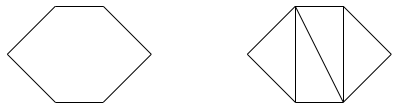
\includegraphics[width=0.5\textwidth]{./Introduction/hex_tri_cells}
\caption{Hexagonal cell versus triangle cells}
\end{figure}
We see that if there is one unknown per vertices, the hexagonal cell has 6
unknowns compared to the 12 unknowns of triangle cells. Polygonal cells can
also be used for adaptive mesh refinement (AMR) problems without having to
deal with hanging nodes \cite{arbitrary_hanging_nodes,dealII_hanging_nodes,
locally_hanging_nodes}. The left cell on the figure below is a pentagon whereas 
the two cells on the right are quadrilaterals:
\begin{figure}[H]
\centering
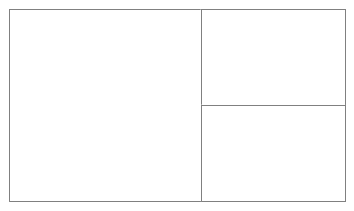
\includegraphics[width=0.3\textwidth]{./Introduction/amr}
\caption{AMR mesh}
\end{figure}
Using MIP requires us to solve SPD equations. This has usually been done using 
conjugate gradient preconditioned by SSOR, but in this research we will test the 
effectiveness of algebraic multigrid methods (AMG) to precondition the Krylov solver 
\cite{amg,amg_course}. Algebraic multigrid methods allow to use multigrid
techniques when there is no grid or that the mesh is unstructured. Instead of
using a succession of grids based on the geometry of the problems, the grids
are based on properties of the matrix. This allows to use AMG as black-box
solvers or preconditioners.

\section{Linear Boltzmann equation}
Charged particles transport can be described by the linear Boltzmann equation 
\cite{morel_81,galerkin_morel,cepxs}:
\begin{equation}
  \begin{split}
    & \bo\cdot \bn \psi(\br,\bo,E) + \Sigma_t(\br,E)\psi(\br,\bo,E) = 
    \int_0^{\infty}dE'\int_{4\pi}d\bo'\ \Sigma_s(\br,\bo'\cdot\bo,E'\rightarrow E)\\
    &\psi(\br,\bo',E')+Q(\br,\bo,E)
  \end{split}
\label{transport_p}
\end{equation}
where:
\begin{itemize}
\item $\bo = (\mu,\varphi)$ is a unit vector in the flight direction
\item $\mu = \cos(\theta)$, where $\theta$ is the directional polar angle
\item $\varphi$ is the directional azimuthal angle
\item $\mu_0 = \bo'\cdot \bo$ is the cosine of the polar angle
\item $\psi(\br,\bo,E) = vf(\br,\bo,E)$ is the angular flux
\item $v$ is the particle speed
\item $\Sigma_t(\br,E)$ is the total macroscopic cross section given by:
\begin{equation}
\Sigma_t(\br,E) = \Sigma_a(\br,E)+\Sigma_s(\br,E)
\end{equation}
\item $\Sigma_a(\br,E)$ is the absorption macroscopic cross section
\item $\Sigma_s(\br,E)$ is the scattering macroscopic cross section
\item $\Sigma_s(\br,\bo'\cdot \bo, E'\rightarrow E)$ is the differential
scattering macroscopic cross scattering
\item $Q(\br,\bo,E)$ is the volumetric source
\end{itemize}
In the rest of this work, macroscopic cross sections will be called cross
sections when no confusion is possible. Standard boundary conditions can be
applied to \cref{transport_p}. The most common is the incoming flux boundary
condition:
\begin{equation}
\psi (\br,\bo,E) = g(\br,\bo,E) \textrm{ for }\bo \cdot \bn <0 \textrm{ and }
\br \in \partial \mc{D}
\label{bc}
\end{equation}
where $\partial \mc{D}$ is the boundary of the domain. If $g=0$, \cref{bc} yields 
the vacuum boundary conditions.

\Cref{transport_p} depends on the space $(\br)$, the angle ($\bo$) and the
energy $(E)$. In this research, we are not interested in the energy variable
and therefore, we will integrate \cref{transport_p} on the energy variable. 
However, the techniques described here apply straightforwardly to the multigroup 
equations. The energy-integrated \cref{transport_p} is given by:
\begin{equation}
\bo\cdot \bn \psi(\br,\bo) + \Sigma_t(\br)\psi(\br,\bo) =
\int_{4\pi}d\bo'\ \Sigma_s(\br,\bo'\cdot\bo)\psi(\br,\bo')+Q(\br,\bo)
\label{transport_p2}
\end{equation}

The in-scattering term can be represented by Legendre polynomials $P_l$ expansion:
\begin{equation}
\begin{split}
\int_{4\pi} \Sigma_s(\br,\bo'\cdot\bo) \psi(\br,\bo') d\bo' &=
\int_{4\pi} \sum_{l=0}^{\infty} \frac{2l+1}{4\pi} \Sigma_{s,l} P_l(\bo'\cdot\bo)
\psi(\br,\bo') d\bo'\\
&= \int_{4\pi} \sum_{l=0}^{\infty} \frac{2l+1}{4\pi}\frac{4\pi}{2l+1}
\Sigma_{s,l}(\br) \times\\
&\quad \sum_{m=-l}^{l} Y_l^m(\bo)Y_l^{m,*}(\bo') \psi(\br,\bo')d\bo'\\
&= \sum_{l=0}^{\infty} \Sigma_{s,l}(\br) \sum_{m=l}^l \phi_{l,m}(\br)
Y_l^m(\bo)
\end{split}
\end{equation}
where we used:
\begin{align}
&\Sigma_s(\br,\bo\cdot\bo') = \sum_{l=0}^{\infty} \frac{2l+1}{4\pi}
\Sigma_{s,l}(\br) P_l(\bo\cdot\bo')\\
&\Sigma_{s,l}(\br) = 2\pi \int_{-1}^1 d\mu_0\ P_l(\mu_0) \Sigma_s(\br,\mu_0)\\
& P_l(\bo\cdot\bo') = \frac{4\pi}{2l+1} \sum_{m=-l}^l
Y_l^m(\bo)Y_l^{m,*}(\bo')\\
& Y_l^m(\bo) = (-1)^m \sqrt{\frac{2l+1}{4\pi} \frac{(l-m)!}{(l+m)!}} P_l^m(\mu)
e^{im\varphi}\\
&\psi(\br,\bo) = \sum_{l=0}^{\infty}\sum_{m=-l}^l \phi_{l,m}(\br) Y_l^m(\bo)
\label{ang_flux}\\
&\phi_{l,m}(\br) = \int_{4\pi} d\bo\ Y_{l}^{m,*}(\bo) \psi(\br,\bo)
\label{moments}
\end{align}
with $Y_l^m$ the spherical harmonics and $P_l^m$ the associated
Legendre polynomials. In practice, the scattering expansion is truncated 
$(\sum_{l=0}^{\infty}\rightarrow \sum_{l=0}^L)$.\\
Later, we will need the following property of the spherical harmonics:
\begin{equation}
\[\frac{\partial}{\partial\mu}(1-\mu^2)\frac{\partial}{\partial
\mu}+\(\frac{1}{1-\mu^2}\)\frac{\partial^2}{\partial \varphi}+l(l+1)\]Y_l^m(\bo)=0
\label{eigenvalue}
\end{equation}
\Cref{transport_p2} still needs to be discretized in space and angle. A
standard method to discretize the space variable is to use discontinuous
Galerkin finite elements \cite{dgfem,thick_dgfem,conv_dgfem}. The angular
discretization that we will use in this work is the $S_n$ or discrete ordinate
method developed in \cite{rad_transfer}. With this discretization, 
\cref{transport_p2} is replaced by a system of linear equations which use discrete 
angular fluxes $\(\psi(\br,\bo)\rightarrow \psi(\br,\bo_d)=\psi_d(\br)\)$ and the 
integral in \cref{moments} is replaced by a quadrature:
\begin{equation}
\phi_{l,m}(\br) = \sum_d w_d Y_{l}^{m,*}(\bo_d) \psi_d(\br)
\label{moments_2}
\end{equation}
where $w_d$ are the weights associated to the quadrature. Therefore, the $S_n$
discretization of \cref{transport_p2} is given by:
\begin{equation}
\bo_d\cdot\bn \psi_d(\br) + \Sigma_t(\br)\psi_d(\br) = \sum_{l=0}^L
\Sigma_{s,l}(\br) \sum_{m=-l}^l \phi_{l,m} Y_l^m(\bo_d) + Q_d(\br)
\label{transport_sn}
\end{equation}
\Cref{transport_sn} can be written in a more compact way:
\begin{equation}
L\Psi = M\Sigma D\Psi + Q
\label{transport_operator}
\end{equation}
where:
\begin{itemize}
\item $L$ is the streaming operator $\bo_d \cdot \bn \bullet + \Sigma_t(\br)
\bullet$
\item $M$ is the moments-to-directions operator $\Psi = M\Phi$
\item $D$ is the directions-to-moments operator $\Phi = D\Psi$
\item $\Sigma$ is the scattering cross-section operator
\end{itemize}


\section{Organization of the Dissertation}
The dissertation is organized as follows.\\

\noindent In Chapter II, we introduce the Boltzmann-Fokker-Planck (BFP)
equation used to describe the transport of charged particles. In the BFP equation
the Fokker-Planck operator is added in the Boltzmann equation in order to simplify
the treatment of the highly forward-peaked scattering kernel. We show that the
Fokker-Planck equation is an asymptotic limit of the Boltzmann equation when the
mean free path goes to zero and $\mu_0$ goes to one. The Fokker-Planck
equation is not valid for every forward-peaked scattering kernel and
therefore, the BFP has limitations. In particular, the Henyey-Greenstein kernel
and the Rutherford cross section do not satisfy the Fokker-Planck equation.
Being aware of these limitations, we introduce the Fokker-Planck cross
section, which allows to reduce the Fokker-Planck equation and the BFP equation
to a Boltzmann equation. Fokker-Planck cross sections cannot be used with any
quadrature, special quadratures known as Galerkin quadratures must be adopted.
The importance and the properties of these quadratures are explained in
details at the end of Chapter II.\\

\noindent In Chapter III, we introduce the angular multigrid methods for 
transport with highly forward-peaked scattering. We recall the previous works 
on the topic and we discuss the problems encountered for multidimensional 
problems. The original angular multigrid method for one-dimensional geometry
shown very quick convergence for problems with highly forward-peaked
scattering whereas DSA is ineffective. Unfortunately, the generalization to
multidimensional geometry required a filter to stabilized the methods which
was not as efficient as in one dimensional geometry. When the scattering
becomes very anisotropic, the angular multigrid method become ineffective. In
that Chapter, we show that if the angular multigrid method is recast as a
preconditioner for a Krylov solver, the method does not need to be stabilized
and is always effective and efficient.\\

\noindent In Chapter IV, we discuss the spatial discretizations: BiLinear
Discontinuous finite elements (BLD) and PieceWise Linear Discontinuous finite
elements (PWLD). The BLD finite elements are used on rectangular cells while
the PWLD finite elements can be used on any polygonal cells. In that Chapter, 
we adapt the Modified Interior Penalty DSA developed for triangular cells to
rectangular and polygonal cells. This DSA discretization is used as the
coarsest level of the angular multigrid method developed in Chapter III. In
Chapter IV, we also investigate algebraic multigrid methods as preconditioners
to solve MIP. Since MIP is symmetric and definite positive (SPD), the most
common method to solve it, is to use conjugate gradient (CG) preconditioned by
SSOR. It is not the only method and we show that CG preconditioned by
algebraic multigrid methods is superior if the matrix associated to MIP can be
stored.\\

\noindent In Chapter V, we finish with some concluding remarks and suggestions for
future developments.

%\section{Transport equation}
Inelastic interactions, collisional and radiative scattering, can be divided
into two classes : ``catastrophic" interactions that result in large-energy
losses and ``soft" interactions that result in small-energy losses. p25 CEPXS

%\section{Fokker-Planck cross section}
In this section, we derive the Fokker-Planck scattering cross section such
that the Fokker-Planck operator can be approximated by the Boltzmann operator.  
First we recall the BFP equation \cref{bfp}:
\begin{equation}
\begin{split}
&\bo\cdot\psi+(\Sigma_{s,reg}+\Sigma_a)\psi=\sum_{l=0}^{\infty}\sum_{m=-l}^l
Y_l^m(\bo)\int_E^{E/\alpha}\Sigma_{s,l,reg}(E'\rightarrow
E)\phi_{l,m}(E')dE'+\\
&\frac{\partial(S\psi)}{\partial E}+\frac{\alpha}{2}\(\frac{\partial}{\partial
\mu}(1-\mu^2) \frac{\partial}{\partial
\mu}+\frac{1}{(1-\mu^2)}\frac{\partial^2}{\partial\varphi^2}\)\psi+Q,
\end{split}
\end{equation}
where we used $\alpha = 2T$.
Let us define:
\begin{align}
\mc{L}_{FP}^{\alpha} \psi &= \frac{\alpha}{2} \frac{\partial}{\partial \mu}
(1-\mu^2) \frac{\partial}{\partial \mu}\psi \label{gamma_alpha}\\
\mc{L}_{FP}^e\psi &=\frac{\partial}{\partial E}S\psi +
\frac{1}{2}\frac{\partial^2}{\partial E^2} R \psi. \label{gamma_e}
\end{align}
We note that $\mc{L}_{FP}^{\alpha}$ causes particles to redistribute in
direction without energy change, while $\mc{L}_ {FP}^e$ causes particles to
redistribute particles in energy without directional change. Therefore,
$\mc{L}_{FP}^{\alpha}$ can be approximated using the following cross section:
\begin{equation}
\Sigma_s(\mu_0,E'\rightarrow E) = \Sigma_s^{\alpha}(\mu_0,E) \delta(E'-E),
\end{equation}
where $\Sigma_{s}^{\alpha} (\mu_0,E) = \frac{\alpha(E)}{1-\mu_s} \frac{1}{2\pi}
\delta(\mu_0-\mu_s)$ and $\mu_s$ is a parameter; while $\mc{L}_{FP}^e$ 
should be approximated by a cross section of the form:
\begin{equation}
\Sigma_s(\mu_0,E'\rightarrow E) = \Sigma_s^e(E'\rightarrow E) \frac{1}{2\pi}
\delta(\mu_0-1).
\end{equation}

\subsection{Legendre polynomial expansion of $\Sigma_s^{\alpha}$}
Next, we express the Legendre polynomial expansion of
$\Sigma_s^{\alpha}(\mu_0)$ ($E$ was dropped for brevity) 
as it has been done in \cite{morel_89,morel_81,morel_96}. We will focus on
$\mc{L}_{FP}^{\alpha}$ since this research we solve the energy-integrated
Boltzmann equation and, therefore, the $\mc{L}_{FP}^e$ operator does not appear in
the equation that we solve. Because $\Sigma_s^{\alpha}$ does not change 
particle energy, it corresponds to a within-group cross section. We define:
\begin{align}
  \mc{L}_B^{\alpha} &= \Sigma_s^{\alpha} \mc{L}_B\\
  \mc{L}_{FP}^{\alpha} &= \frac{\alpha}{2}\mc{L}_{FP},
\end{align}
and thus:
\begin{align}
\mc{L}_B^{\alpha}Y_l^m(\bo) &= (\Sigma_{s,l}^{\alpha}-\Sigma_{s,0}^{\alpha})
Y_l^m(\bo) \label{gamma_b_alpha_p}\\
\mc{L}_{FP}^{\alpha} Y_l^m(\bo) &= -\frac{\alpha}{2} l(l+1) Y_l^m(\bo).
\label{gamma_fp_alpha_p}
\end{align}
Using \cref{ang_flux,gamma_b_alpha_p,gamma_fp_alpha_p}, we can define 
$\Sigma_s^{\alpha}$ such that:
\begin{equation}
\mc{L}_B^{\alpha}\psi=\mc{L}_{FP}^{\alpha}\psi,
\end{equation}
by setting:
\begin{equation}
\Sigma_{s,l}^{\alpha}-\Sigma_{s,0}^{\alpha} = -\frac{\alpha}{2}l(l+1),
\label{sigma_m_sigma}
\end{equation}
with $l=1,\hdots,L$. Choosing $\Sigma_{s,L}^{\alpha}=0$ to minimize 
$\Sigma_{s,0}^{\alpha}$ and \cref{sigma_m_sigma} becomes:
\begin{equation}
\Sigma_{s,l}^{\alpha} = \frac{\alpha}{2}\(L(L+1)-l(l+1)\),\ \  l=0,\hdots,L.
\label{eq_297}
\end{equation}
Using appropriate quadrature sets and expansion orders, the $S_n$
representation of $\mc{L}_{FP}^{\alpha}$ is equivalent to the one obtained by
interpolating the discrete angular flux values with a polynomial.

Next, we look at the behavior of $\Sigma_s^{\alpha}$ when the degree of the expansion 
is increased. First, we should note that the momentum transfer of
$\Sigma_s^{\alpha}$ is exact for any expansion order:
\begin{equation}
\begin{split}
2\pi \int_{-1}^1 \Sigma_s^{\alpha}(\mu_0) (1-\mu_0) d\mu_0 &=
\Sigma_{s,0}-\Sigma_{s,1}\\
&=\frac{\alpha}{2} L(L+1) - \frac{\alpha}{2} (L(L+1)-2)\\
&=\alpha.
\end{split}
\end{equation}
With \cref{eq_297}, the average cosine of the scattering angle
becomes:
\begin{equation}
\begin{split}
\bar{\mu}_0 &= \frac{\Sigma_{s,1}^{\alpha}}{\Sigma_{s,0}^{\alpha}}\\
&=\frac{L(L+1)-2}{L(L+1)}.
\end{split}
\end{equation}
It is easily seen that when $L$ increases, $\bar{\mu}_0$ goes to one and
$\Sigma_s^{\alpha}$ becomes increasingly forward-peaked. The
total magnitude of $\Sigma_s^{\alpha}(\mu_0)$ becomes unlimited when $L$ goes to
$\infty$:
\begin{equation}
\Sigma_{s,0}^{\alpha} = \frac{\alpha}{2} L (L+1).
\end{equation}
This shows that $\mc{L}_{FP}^{\alpha}$ corresponds to a continuous-deflection 
interaction. The particles are continuously 
deflected with the mean deflection per unit pathlength given by the momentum transfer.

$\mc{L}_{B}^{\alpha}$ converges to $\mc{L}_{FP}^{\alpha}$ when $\mu_s$ tends
to one but it does not converge uniformly. For any fixed value of $\mu_s$, 
the high-order eigenvalues of $\mc{L}_{FP}^{\alpha}$ are grossly underestimated 
by $\mc{L}_B^{\alpha}$. Fortunately, this is error in the high-order eigenvalues 
is usually unimportant \cite{morel_96}.

%\section{Galerkin quadratures}
Until now, we have not described which angular quadrature should be used to
correctly treat high orders of anisotropy. We have only
stated that we need an appropriate quadrature but we did not explain what we
required. In this section, we introduce the Galerkin quadrature. Morel
first introduced them in \cite{galerkin_morel}; here, we
will introduce them following the presentation made in \cite{pautz_fp}. 

First, we start by recalling the definition of $\psi$ and $\phi_{l,m}$:
\begin{equation}
  \begin{split}
    \phi_{l,m}(\br) &= \int_{4\pi} d\bo' \psi(\br,\bo') Y_l^{m,*}\\
                    &=(\bs{D} \Psi)_{l,m}
  \end{split}
  \label{D2M}
\end{equation}
where $\bs{D}$ is the direction-to-moment operator. We also have:
\begin{equation}
  \begin{split}
    \Psi(\br,\bo) &= \sum_{l=0}^{\infty} \sum_{m=-l}^l Y_l^m(\bo)\phi_{l,m}(\br)\\
                  &= \bs{M}\Phi(\br)
  \end{split}
  \label{M2D}
\end{equation}
where $\bs{M}$ is the moment-to-direction operator. By combining \cref{D2M,M2D}, 
we obtain:
\begin{equation}
  (\bs{I}-\bs{MD})\Psi = 0
  \label{identity_alpha}
\end{equation}
since for analytic transport $\bs{M}=\bs{D}^{-1}$. $\bs{I}$ is the identity operator.

Now, we define \cite{pautz_fp}:
\begin{align}
\epsilon &= 1 - \la \bar{\mu}_0\ra \label{eps_pautz} \\
    \gamma &= \la\overline{(1-\mu_0)^2}\ra \label{gamma_pautz}\\
    A(\br) &= \frac{1-\bar{\mu}_0(\br)}{\epsilon}\label{A_pautz}\\
  \Sigma_a &= \hat{\Sigma}_a \label{hat_sig_a_0}\\
\Sigma_{s,l} &= \frac{\hat{\Sigma}_{s,l}(\br)}{\epsilon} \label{hat_sig_a_1}\\
\Sigma_{s,l}(\br) &=\Sigma_{s,0}(\br) \(1-\frac{l(l+1)}{2}A(\br)\epsilon +
  O(\gamma)\) \label{hat_sig_a_2}
\end{align}
where $\la X \ra$ is a typical value of $X$. Using \crefrange{eps_pautz}{hat_sig_a_2} 
in \cref{transport_sn}, we get:
\begin{equation}
\begin{split}
&\bo_k\cdot\bn\psi_k(\br) + \(\Sigma_a(\br)+\Sigma_{s,0}(\br)\) \psi_k(\br)
=\\
& \sum_{l=0}^{N-1} \sum_{m=-l}^l Y_l^m(\bo_k) \phi_{l,m}(\br)
\frac{\hat{\Sigma}_{s,0}(\br)}{\epsilon}\(1-\frac{l(l+1)}{2}A(\br)\epsilon +
O(\gamma)\) + Q(\br,\bo_k)
\end{split}
\label{discr_eps}
\end{equation}
where:
\begin{align}
\psi_k(\br) &= \psi(\br,\bo_k)\\
\phi_{l,m}(\br) &= \sum_{k=1}^K w_k Y_l^{m,*}(\bo_k) \psi_k(\br). \label{phi_p}
\end{align}
$w_k$ and $\bo_k$ are the quadrature weights and directions of a 
quadrature set of order $N$. For triangular quadrature sets, $K=N$ in 1D, 
$K=\frac{N(N+2)}{2}$ in 2D and $K=N(N+2)$ in 3D. \Cref{discr_eps} yields:
\begin{equation}
\begin{split}
&\bo_k\cdot\bn \psi_k(\br) +\hat{\Sigma}_a(\br)\psi_k(\br)+
\frac{\hat{\Sigma}_{s,0}(\br)}{\epsilon} \(\psi_k(\br)-\sum_{l=0}^{N-1}
\sum_{m=-l}^m  Y_l^m(\bo_k) \phi_{l,m}\)\\
&=-\frac{\(\Sigma_{tr}(\br)-\hat{\Sigma}_a(\br)\)}{2} \sum_{l=0}^{N-1}
\sum_{m=-l}^{l} l(l+1) Y_l^m(\bo_k) \phi_l^m(\br)+
 Q(\br,\bo_k) + O\(\frac{\gamma}{\epsilon}\).
\end{split}
\label{discr_eps_manip}
\end{equation}
We insert the asymptotic ansatz:
\begin{align}
\psi &= \psi^{(0)} + \epsilon \psi^{(1)} + \epsilon^2\psi^{(2)}+\hdots\\
\phi_{l,m} &= \phi_{l,m}^{(0)} + \epsilon \phi_{l,m}^{(1)} + \epsilon^2
\phi_{l,m}^{(2)}+\hdots
\end{align}
into \cref{discr_eps}. The terms of $O(1)$ give:
\begin{equation}
\begin{split}
\phi_{l,m}^{(0)}(\br) &= \sum_{k=1}^K w_k Y_l^{m,*}(\bo_k) \psi_k^{(0)}(\br)\\ 
                      &= (\bs{D}_N\Psi^{(0)})_{l,m}.
\end{split}
\label{D2M_disc}
\end{equation}
Now we insert the ansatz into \cref{discr_eps_manip} and we look at the terms
of $O(\epsilon^{-1})$:
\begin{equation}
\begin{split}
\psi_d^{(0)}(\br) &=\sum_{l=0}^{N-1} \sum_{m=-l}^l Y_l^m(\bo_k) 
\phi_{l,m}^{(0)}(\br)\\
&= (\bs{M}_N\Phi^{(0)})_d
\end{split}
\label{M2D_disc}
\end{equation}
there is no $O(\gamma)$ term, since $\gamma\rightarrow 0$ when 
$\epsilon\rightarrow 0$, i.e., that there are no
$O(1)$ components in $\gamma$. \Cref{D2M_disc,M2D_disc} may be combined to give:
\begin{align}
  &(\bs{I}-\bs{M}_N\bs{D}_N)\Psi^{(0)} = 0 \label{identity_a}\\
  &(\bs{I}-\bs{D}_N\bs{M}_N)\Phi^{(0)} = 0 \label{identity_b}.
\end{align}
This means that $\Psi^{(0)}$, respectively $\Phi^{(0)}$, must be in the kernel
of $\bs{I}-\bs{M}_N \bs{D}_N$, respectively $\bs{I}-\bs{D}_N \bs{M}_N$. Using 
\cref{phi_p}, \cref{identity_b} becomes successively:
\begin{equation}
  \(\bs{I}-\bs{D}_N \bs{M}_N\) \bs{D}_N \Psi^{(0)} = 0
\end{equation}
\begin{equation}
  \(\bs{D}_N-\bs{D}_N \bs{M}_N \bs{D}_N\) \Psi^{(0)} = 0
\end{equation}
\begin{equation}
  \bs{D}_N(\bs{I}-\bs{M}_N \bs{D}_N)\Psi^{(0)} = 0,
\end{equation}
which is always satisfied if \cref{identity_a} is satisfied.
Therefore, if \cref{identity_a} is satisfied, \cref{D2M_disc,M2D_disc} are
automatically satisfied.

A sufficient condition to satisfy \cref{identity_a} is that $\bs{M}_N \bs{D}_N
=\bs{I}$. This is of course true if $\bs{D}_N=\bs{M}_N^{-1}$ like in analytic 
transport. Obviously for $\bs{M}_N$ and $\bs{D}_N$ to be inverse of each other, 
the matrices have to be square. Thus, the number of moments in the scattering 
expansion must be equal to number of discrete angles. In one-dimension,
$\bs{D}_N = \bs{M}_N^{-1}$ is satisfied if the 
quadrature set integrates exactly any polynomials of degree $2N-1$, like the 
Gauss-Legendre quadrature does. In multidimensional problems, the standard 
quadrature sets use more discrete angles than there are scattering moments. 
Therefore, $\bs{M}_N$ and $\bs{D}_N$ are rectangular matrices and they cannot 
be inverse of each other. In this case, \cref{identity_a} can only be satisfied if 
$\Psi^{(0)}$ is in the kernel of $(\bs{I}-\bs{M}_N\bs{D}_N)$. This can be achieved 
only if $\Psi^{(0)}$ satisfies nonphysical constraints \cite{pautz_fp}. If 
\cref{identity_a} is not satisfied, the asymptotic ansatz is not valid and 
there is no $O(1)$ solution to \cref{discr_eps,phi_p}.\\
If we assume that $\bs{M}_N \bs{D}_N=\bs{I}$, then the $O(\epsilon)$ terms in 
\cref{phi_p} give:
\begin{equation}
  \begin{split}
    \phi_{l,m}^{(1)}(\br) &= \sum_{k=1}^K w_k Y_{l}^{m,*} (\bo_k) \psi_k^{(1)}(\br)\\
                          &=(\bs{D}_N\Psi^{(1)})_{l,m}
  \end{split}
\end{equation}
In \cref{discr_eps_manip}, the $O(1)$ terms give:
\begin{equation}
  \begin{split}
    &\bo_k\cdot \bn \psi_k^{(0)}(\br) + \hat{\Sigma}_a(\br)\psi_k^{(0)}(\br) +
    \hat{\Sigma}_{s,0}(\br) \(\psi_k^{(1)} (\br) - \sum_{n=0}^{N-1}
    \sum_{m=-l}^{l} Y_l^m (\bo_k)\phi_{l,m}^{(1)}(\br)\)\\
    &=-\frac{\Sigma_{tr}(\br)-\hat{\Sigma}_a(\br)}{2} \sum_{l=0}^{N-1}
    \sum_{m=-l}^l  l(l+1) Y_l^m(\bo_k)
    \phi_{l,m}^{(0)}(\br)+ Q(\br,\bo_k) + O\(\frac{\gamma}{\epsilon}\).
  \end{split}
  \label{O_1_terms}
\end{equation}
Now, we want the scattering term on the left side of \cref{O_1_terms} to
disappear in order to keep only $\psi_k^{(0)}$ and $\phi_{l,m}^{(0)}$. This 
is possible only if:
\begin{equation}
\psi_d^{(1),*}(\br) = \psi_d^{(1)}(\br)
\label{psi_1_star_old}
\end{equation}
where:
\begin{equation}
  \begin{split}
    \psi_d^{(1),*} &= \sum_{l=0}^{N-1}\sum_{m=-l}^l Y_l^m(\bo_k) 
    \phi_{l,m}^{(1)}(\br)\\
                   &= (\bs{M}_N\Phi^{(1)})_d\\
                   &=(\bs{M}_N \bs{D}_N \Psi^{(1)})_d
  \end{split}
  \label{psi_1_star}
\end{equation}   
which is satisfied because of our previous assumption that $\bs{M}_N \bs{D}_N
= \bs{I}$. \Cref{O_1_terms} yields:
\begin{equation}
\begin{split}
  &\bo_k \cdot \bn \psi_k^{(0)}(\br)+\hat{\Sigma}_a(\br) \psi_k^{(0)}(\br) =
  \frac{\Sigma_{tr}(\br)-\hat{\Sigma}_a(\br)}{2}
  \(\(\frac{\partial}{\partial \mu}(1-\mu^2)\frac{\partial}{\partial
  \mu}+\right. \right.\\
  &\left.\left. \(\frac{1}{1-\mu^2}\)\frac{\partial^2}{\partial \varphi^2}\)
  \tilde{\psi}^{(0)} (\br,\bo)\)_{\bo=\bo_k}+ Q(\br,\bo_k) + 
  O\(\frac{\gamma}{\epsilon}\)
\end{split}
\label{last_pautz}
\end{equation}
where $k=1,\hdots,K$ and $\tilde{\psi}^{(0)}(\br,\bo)$ is an interpolant
through the points $P_k=\{\bo_k,\psi_k^{(0)}(\br,\bo)\}$. ``In one-dimensional 
geometry, $\tilde{\psi}^{(0)}(\br,\bo)$ is the $(N-1)-$order
polynomial interpolant through the points $P_k$. In multidimensional
geometries, $\tilde{\psi}^{(0)}(\br,\bo)$ is the spherical harmonic
interpolant through the points $P_k$'' \cite{pautz_fp}. A quadrature which 
satisfies the relation $\bs{D}_N = \bs{M}_N^{-1}$ is called a ``Galerkin'' quadrature 
because Morel derived it by using a Galerkin weighting method \cite{galerkin_morel}.

In \cite{galerkin_morel}, Morel made the following suggestions to find the 
correct limit using the $S_N$:
\begin{description}
\item [One-dimensional geometry:] The Gauss-Legendre quadrature set is the
  only quadrature set which is a Galerkin quadrature.
\item [Multidimensional geometry:] The standard quadrature sets have fewer 
  moments than discrete angles. Therefore to satisfy $\bs{D}=\bs{M}^{-1}$, spherical
  harmonics of higher order need to be added to increase the number of moments
  up to the number of angular flux. Morel in \cite{galerkin_morel} and Reed in 
  \cite{reed} proposed an heuristic algorithm to choose the spherical 
  harmonics for multidimensional geometries. If we use the real spherical
  harmonics defined by:
  \begin{equation}
    Y_{l,m}^c = \left\{
      \begin{aligned}
        &Y_l^0 & \textrm{ if } m=0\\
        &\frac{1}{\sqrt{2}} \(Y_l^m+(-1)^{m} Y_l^{-m}\) & \textrm{ if } m> 0
      \end{aligned}
      \right.
  \end{equation}
  \begin{equation}
    Y_{l,m}^s = \frac{1}{i\sqrt{2}}(Y_l^{-m}-(-1)^{m}Y_l^m) \textrm{ if } m<0
  \end{equation}
  and a two-dimensional triangular quadrature set, the selection rules to build 
  $\bs{M}$ are the following:
  \begin{itemize}
    \item Take $Y_{l,m}^c$ if $l\in[0,N-1]$, $m\in[0,l]$, and $l+m$ is even.
    \item Take $Y_{l,m}^s$ if ($l \in [1,N-1]$, $m\in[1,l]$, and $l+m$ is
      even) or if ($l=N$, $m\in[1,l]$, and $l+m$ is even).
  \end{itemize}
  For three dimensional triangular quadrature sets, the spherical harmonics
  are:
  \begin{itemize}
    \item Take $Y_{l,m}^c$ if ($l \in [0,N-1]$ and $m\in[0,l]$) or if ($l =
      N$, $m\in[1,N-1]$, and $m$ is odd).
    \item Take $Y_{l,m}^s$ if ($l\in [1,N]$ and $m\in[1,l]$) or if ($l=N+1$,
      $m\in[2,N]$ and $m$ is even).
  \end{itemize}
\end{description}
General necessary conditions and explanations of the heuristic rules above
have been analyzed in \cite{galerkin_sanchez}.

Using a standard $S_n$ quadrature may led to an unphysical solution for
charged particle transport. To further demonstrate the importance of Galerkin
quadrature, we define the scattering ratio matrix $\bs{C}$ by:
\begin{equation}
\bs{C} = \frac{1}{\Sigma_t}\bs{D}\bs{M}\bs{\Sigma},
\end{equation}
where $\bs{\Sigma}$ is the scattering matrix containing the moments of the
scattering cross sections on its diagonal.
$\bs{C}$ is a diagonal matrix whose entries are the scattering ratios
$c_l=\frac{\Sigma_{s,l}}{\Sigma_t} \leq 1$. The fact that $\bs{MD}=\bs{I}$
assures a one-to-one relation between the angular flux and the flux moments;
furthermore, the orthogonality of all spherical harmonic functions used in the
angular flux representation is preserved. However, if a standard quadrature is
employed, then $\bs{D} = \bs{M}^T \bs{W}$, where $\bs{W}$ is the diagonal
matrix of weights, and inexact integration occurs for the set of spherical
harmonics than span $\bs{M}$. Thus, $\bs{C}$ will differ from
$\frac{\bs{\Sigma}}{\Sigma_t}$ and its eigenvalue could exceed unity. This is
equivalent to numerically adding multiplication into the medium and, depending
on the amount of leakage present in the geometrical configuration, the
steady-state transport equation may not reach a steady state solution
\cite{pautz_fp}.

A very important property of the Galerkin quadratures is that they treat the
delta function scattering exactly. This is very important for two reasons. 
The first reason is that in charged-particle transport, some cross sections 
have the following form:
\begin{equation}
\Sigma^{k\rightarrow g}(\mu_0) = \Sigma^{k\rightarrow g} \delta(\mu_0-1),
\end{equation}
where $\Sigma^{k\rightarrow g}(\mu_0)$ is the differential cross section
associated with a transfer from group $k$ to group $g$. Thus, it is essential
that delta function scattering be treated exactly. The second reason, which is
more important for us since we work with energy-integrated equation, is that for 
electron scattering, the extended transport correction \cite{lathrop} can be 
used to reduce the within-group scattering cross sections by two orders of 
magnitude or more \cite{morel_79}. Without the extended transport correction, 
the high order of the flux moments are very important and DSA does not 
accelerate the convergence of the solver. Because the Galerkin method treats 
delta function  scattering exactly, the extended transport correction does not
modify the solution of the problem \cite{morel_79}. This is very interesting 
since it allows to reduce significantly the higher moments of the scattering
cross-section expansion without losing of accuracy. Showing this property is
quite simple given what we have presented thus far. We know that in the analytic case
we have:
\begin{equation}
\int_{4\pi} \delta(\mu_0-1) \psi(\bo')\ d\bo' = \psi(\bo).
\end{equation}
When the scattering source is discretized, we have $\bs{\Sigma}=\bs{I}$.
Therefore, it is obvious that:
\begin{equation}
  \bs{D\Sigma M}\Psi = \Psi.
\end{equation}

To really understand the Galerkin quadrature, it is interesting to recall 
the development made in \cite{galerkin_morel}. First, we expand the
one-dimensional angular flux on an interpolatory trial space:
\begin{equation}
\Psi(\mu) = \sum_{d=1}^N \psi_d B_d(\mu).
\label{psi_b}
\end{equation}
Methods for generating the interpolatory basis function can be found in 
\cite{galerkin_morel}. Next, we expand the scattering source on the Legendre
polynomials:
\begin{equation}
\mc{S}(\mu) = \sum_{l=0}^{\infty} \frac{2l+1}{2} \xi_l P_l(\mu)
\label{S_mu_2}
\end{equation}
where:
\begin{equation}
  \xi_l = \int_{-1}^1 \mc{S}(\mu) P_l(\mu) d\mu.
\end{equation}
Now, we use the interpolatory trial space to approximate $S(\mu)$:
\begin{equation}
\tilde{\mc{S}}(\mu) = \sum_{d=1}^N \tilde{\mc{S}}_d B_d(\mu)
\label{tilde_s_mu}
\end{equation}
Since a Galerkin method is used, the residual associated with the trial space 
approximation must be orthogonal to the weighting
space. The residual associated with \cref{tilde_s_mu} is given by:
\begin{equation}
Res(\mu) = \tilde{\mc{S}}(\mu) - \mc{S}(\mu).
\label{R_mu}
\end{equation}
Since the Legendre polynomials form a basis the weighting space, we
orthogonalize against the Legendre polynomials:
\begin{equation}
\int_{-1}^1 Res(\mu) P_l(\mu) d\mu = 0.0,\ \ l=0,\hdots,N-1.
\label{int_r_mu}
\end{equation}
\Cref{int_r_mu} is satisfied if:
\begin{align}
&\tilde{\xi}_l = \xi_l,\ \ l=0,\hdots,N-1 \label{xi_vs_xi}\\
&\tilde{\xi}_l = \int_{-1}^1 \tilde{\mc{S}}(\mu) P_l(\mu) d\mu.
\end{align}
The main idea of the Galerkin quadrature can be seen on \cref{xi_vs_xi}: ``the
discrete scattering source values are chosen such that the interpolatory
representation for that scattering source has the same Legendre moments
through degree $N-1$ as the exact scattering source calculated with the
interpolatory representation for the angular flux \cite{galerkin_morel}''. 
Because all the elements of the weighting space can be expressed as a linear
combination of Legendre polynomials $P_l$ with $l<N$ and $\int_{-1}^{1}
P_l(x)P_m(x)\ dx=0$ for $l\neq m$, only the first $N-1$ cross-section moments
are needed.

Now, we compare the cross-section expansion for the Galerkin method and
the $S_n$ method. Both the Galerkin method and the standard $S_n$ method use
the Legendre expansion of the cross section. However, whereas the $S_n$ method
actually uses the Legendre expansion, the Galerkin scattering source is
fully consistent with the exact cross section. It is not
important whether or not the Legendre cross-section expansion represent
accurately the scattering cross section. What is important is that
$\tilde{S}(\mu)$ is an accurate approximation of $S(\mu)$. This is a crucial 
property for charged particle transport. For example, the delta
function expansion of finite degree is never converged, and this is an issue if a 
$S_n$ method with a standard quadrature is used. However, as proved earlier, 
the scattering source computed by the Galerkin method is treated exactly.

If the scattering is isotropic, the $S_n$ method appears superior to the
Galerkin, since the Galerkin requires the number of flux moments to be equal
to the number of angular flux. Fortunately, if the higher order cross-sections
moments are zero, only the first rows of $\bs{D}$ and the first columns of
$\bs{M}$ need to be kept.

A Galerkin quadrature set and its companion quadrature sets (standard
quadrature sets associated to the Galerkin quadrature set) are different only
if the expansion order of the scattering cross section is high enough. When the 
scattering is isotropic, the Galerkin quadrature set is the same than its
companion set. Even when the scattering is highly anisotropic, the results
given by the Galerkin set and its companion set can be very close. This is due
to the fact the high order moments of the scattering cross section are often,
but not always, very small.

%\section{Iterative schemes for highly forward-peaked scattering}
\subsection{Source Iteration and DSA}
\Cref{transport_operator} can be solved using the Source Iteration 
method, which is a Richardson iteration, or a Krylov method. The Source
Iteration method at the $k^{th}$ iteration is given by:
\begin{equation}
\Phi^{(k+1)} = \bs{DL}^{-1} \bs{M\Sigma}\Phi^{(k)}+\bs{DL}^{-1}Q
\end{equation}
When the scattering ratio $c=\max_{l}\(\frac{\Sigma_{s,l}}{\Sigma_t}\)$ is close
to one, the spectral radius of SI can become arbitrary close to one and the
convergence becomes arbitrary slow. Since
most physical forward-peaked scattering produces $\Sigma_{s,0} >
\Sigma_{s,1}>\hdots$, the flat modes are the ones which should be accelerated
that is why the DSA scheme is used. The SI+DSA scheme is given by a transport sweep:
\begin{equation}
\Phi^{(k+1/2)} = \bs{DL}^{-1}\bs{M\Sigma}\Phi^{(k)} +\bs{DL}^{-1}Q,
\label{dsa_sweep}
\end{equation}
followed by a diffusion synthetic acceleration for the correction:
\begin{equation}
\delta \Phi^{(k)} = \bs{\mc{T}}_0^{-1} \bs{R}_{n\rightarrow0}
\(\Phi^{(k+1/2)}-\Phi^{(k)}\),
\label{correction}
\end{equation}
yielding the next iterate for the flux moments:
\begin{equation}
\Phi^{(k+1)} = \phi^{(k+1/2)} + \bs{P}_{0/1\rightarrow n} \delta \Phi^{(k)}
\label{si_dsa_it}
\end{equation}
Finally, using \crefrange{dsa_sweep}{si_dsa_it}, we obtain:
\begin{equation}
\begin{split}
\Phi^{(k+1)} =& \((\bs{I}+\bs{P}_{0/1\rightarrow n}\bs{\mc{T}}_0^{-1} \bs{R}_{n
\rightarrow 0}\bs{DL}^{-1} \bs{M\Sigma} - \bs{P}_{0/1\rightarrow n}
\bs{\mc{T}}_0^{-1} \bs{R}_{n\rightarrow 0}\) \Phi^{(k)}\\
&+ (\bs{I} + \bs{P}_{0/1\rightarrow n}\bs{\mc{T}}_0^{-1} \bs{R}_{n\rightarrow
0}) \bs{DL}^{-1} Q.
\end{split}
\label{dsa_it}
\end{equation}
where $\bs{\mc{T}}_0$ is the matrix associated to the DSA operator,
$\bs{R}_{n\rightarrow 0}$ is the restriction matrix of $\Phi_n$ (all moments)
to $\Phi_0$ (only $0^{th}$ moment) and $\bs{P}_{0/1\rightarrow n}$ the
projection matrix of $\Phi_0$ or $\Phi_1$, depending whether only the zeroth
or the zeroth and the first moment are accelerated, onto $\Phi_n$. When only
the zeroth moment is accelerated, the scheme is always stable and the spectral
radius is max $\(\rho_{iso},\frac{\Sigma_{s,1}}{\Sigma_t}\)$ where
$\rho_{iso}$ is the spectral radius when the scattering is isotropic. In
multidimensional geometry, when both the zeroth and the first moments are
accelerated, the scheme is not always stable and the spectral radius is given
by $\(\rho_{iso},\frac{\Sigma_{s,1}}{\Sigma_{t}-\Sigma_{s,1}}\)$
\cite{multisweep}. For highly forward peaked scattering, accelerating the
zeroth moment is ineffective $\(\frac{\Sigma_{s,1}}{\Sigma_t}\rightarrow 1\)$,
whereas accelerating both moments can be unstable
$\(\frac{\Sigma_{s,1}}{\Sigma_t-\Sigma_{s,1}}>1\)$.

\section{Review of previous angular multigrid work}
\subsection{One dimensional geometry: the Morel and Manteuffel (MM) method}
As mentioned previously, only the zeroth and the first flux moments can be
accelerated with DSA. To accelerate higher moments, other methods have to be
used. Morel and Manteuffel proposed an angular multigrid method to accelerate
the SI calculation of the one-dimension $S_n$ equations with highly
anisotropic scattering \cite{multigrid_1d}. They use a variation of the
extended transport correction \cite{lathrop} to attenuate the ``upper half''
of the flux moments (higher frequencies) thanks to transport sweeps. The
``lower half'' of the flux moments (lower frequencies) is accelerated using
the $S_{n/2}$ equations. These $S_{n/2}$ equations are themselves accelerated
using $S_{n/4}$ equations. The order of the transport operator is divided
by two until the $S_4$ level. At this point, the $P_1$ equations are used to
accelerate the $S_4$ equations. For the general case where $n/2^i$ is odd, we need
to define:
\begin{equation}
Half(n) = \left\{
\begin{aligned}
&\frac{n}{2}, &\textrm{if }\frac{n}{2}\textrm{ is even}\\
&\frac{n}{2}+1, &\textrm{if }\frac{n}{2}\textrm{ is odd}
\end{aligned}
\right.
\end{equation}
Using this definition of ``Half'' to coarsen the angular grid, the sequence of
sweeps for an $S_{16}$ base level is $(S_{16}-S_8-S_4)$ and for a $S_{18}$
base level, the sequence is $(S_{18}-S_{10}-S_6-S_4)$. Morel and Manteuffel's
scheme works as follows:
\begin{enumerate}
\item Perform a transport sweep for the $S_n$ equations.
\item Perform a transport sweep for the $S_{n_2}$ equations with a $P_{n_2-1}$
expansions using the $S_n$ residual as the inhomogeneous source, where
$n_2=Half(n)$.
\item Continue coarsening the angular grid by a factor two (i.e., according to
the definition of ``Half'') until a sweep has been performed for the $S_4$
equations.
\item Solve the $P_1$ equations ($P1$ synthetic acceleration, $P1SA$) with a
$P_1$ expansion of the $S_4$ residual as the inhomogeneous source.
\item Add the Legendre moments of the $P_1$ solution to the Legendre moments
of the $S_4$ iterate to obtain the accelerated $S_4$ iterate.
\item Continue to add the corrections from each coarse grid to the finer grid
above to obtain the accelerated $S_n$ moments.
\end{enumerate}
Every time a transport sweep is performed, the optimal transport correction
needs to be used \cite{multigrid_1d}. For a $P_{n-1}$ expansion of the cross
sections, the corrected cross sections are given by:
\begin{equation}
\Sigma_{s,j}^* = \Sigma_{s,j} - \frac{\Sigma_{s,n/2}+\Sigma_{s,n-1}}{2}
\textrm{with }j=\{t\}\textrm{ or }\{s,l\}.
\end{equation}
This correction is said to be optimal because for an infinite homogeneous
medium, it minimizes the ``high-frequency'' angular errors, the smoothing
factor being given by:
\begin{equation}
\rho_s =\max\(|\Sigma_{s,n/2}|/\Sigma_{s,0},|\Sigma_{s,n/2+1}|/\Sigma_{s,0},
\hdots,|\Sigma_{s,n-1}|/\Sigma_{s,0}\).
\label{rho_s}
\end{equation}
To compare the effectiveness of the angular multigrid method with DSA,
Fokker-Planck scattering cross sections (\cref{sigma_m_sigma}) can be used. In
one dimension geometry, DSA becomes less efficient as $\Sigma_{s,l}$ $(0<l\leq
L)$ becomes closer to $\Sigma_{s,0}$. Therefore, in the limit as $L\rightarrow
\infty$, DSA no longer accelerates the convergence of SI for Fokker-Planck
scattering (the spectral radius tends to 1.0). However, the spectral radius of
the angular multigrid method has an upper bound of $0.6$ when $L\rightarrow
\infty$. It can be easily shown by using \cref{rho_s} and the fact that for
Fokker-Planck scattering cross sections the cross-section moments decrease
monotonically:
\begin{equation}
  \begin {split}
  \rho_s &= \frac{\Sigma_{s,N/2}^*}{\Sigma_{s,0}}\\
         &= \frac{3N-6}{5N-6}
  \end{split}
\end{equation}
which tends to 0.6 when $N$ goes to infinity.

The MM method converges in less iterations than DSA but it is important to
look at the cost of each MM iterations: one sweep in each $N$ directions + one
DSA iteration + one sweep in each ($\frac{N}{2}+\frac{N}{4}+\hdots$)
directions. Since $\frac{N}{2}+\frac{N}{4}+\hdots \leq N$, the cost of one MM 
iteration is less than: two sweeps in each $N$ directions + one DSA iteration.

\subsection{Multidimensional geometry: the Pautz-Adams-Morel (PAM) methods}
In the multidimensional case, DSA becomes unstable when both the zeroth and
the first flux moments are accelerated and $\frac{\Sigma_{s,1}}{\Sigma_t}\geq
0.5$, \cite{multisweep}. In \cite{multigrid_2d}, the authors modified the one
dimensional angular multigrid method by accelerating only the zeroth flux
moment with the DSA and by using $S_2$ as lowest transport sweep instead of
$S_4$. Even so, the proposed method (PAMNF, with ``NF'' for no-filtering) was
unstable and a filter was needed to stabilize the scheme (PAMF). Therefore,
the angular multigrid method was modified as follows \cite{multigrid_2d}:
\begin{enumerate}
\item Perform a transport sweep for the $S_n$ equations.
\item Perform a transport sweep for the $S_{n_2}$ equations with a $P_{n_2}$
for 2-D problem and a $P_{n_2+1}$ for 3-D problem expansion for the $S_n$
residual as the inhomogeneous source, where $n_2 = Half(n)$.
\item Continue coarsening the angular grid by a factor two (i.e., according to
the definition of ``Half'') until a sweep has been performed for the $S_2$
equations.
\item Solve the diffusion equation with a $P_0$ expansion for the $S_2$
residual as the inhomogeneous source.
\item Apply a diffusive filter to the corrections from steps 2 and 3 (without
this, the method is unstable).
\item Add the corrections from steps 4 and 5 to the Legendre moments of the
$S_n$ iterate to obtain the accelerated $S_n$ moments.
\end{enumerate}
The filter stabilizes the method which otherwise would diverge. Without the
filtering process, the low frequency are well attenuated but instabilities are
introduced in higher frequency modes. Filtering eliminates the high frequency
corrections which are well attenuated by SI alone but it keeps the low
frequency corrections. The filter is given by:
\begin{equation}
\(-\bn\cdot \frac{\beta_f}{3\Sigma_f}\bn + \Sigma_f\) f_{corr} = \Sigma_f
\(\Phi_{n_2}+P_{n_4\rightarrow n_2}\Phi_{n_4}+\hdots+P_{2\rightarrow
n_2}\Phi_2\)
\end{equation}
where $\Sigma_f$ is the filter cross section and $\beta_f$ is the filter
tuning parameter. A Fourier analysis shows that given an input amplitude $A$,
the ``diffusively filtered'' amplitude is:
\begin{equation}
F=\frac{A}{1+\frac{\beta_f \lambda^2}{3\Sigma_f}}.
\end{equation}
It is clear that the modes with large $|\lambda|$ (high frequencies) are
strongly attenuated while low-frequency are not. However, the filtering
process does not prevent the spectral radius from becoming arbitrary close to
1 when $L$ becomes large \cite{multigrid_2d}.

\section{Angular multigrid as preconditioner for Krylov Solvers}
In this research, we propose to abandon SI as the solver for the $S_n$
equations with highly-forward peaked scattering and to use a Krylov solver
instead. The DSA-preconditioned system of equations solved with a Krylov method is:
\begin{equation}
\begin{split}
&\((\bs{I} + \bs{P}_{0/1\rightarrow n} \bs{\mc{T}}_0^{-1} \bs{R}_{n\rightarrow
0})(\bs{I}-\bs{DL}^{-1}\bs{M\Sigma})\) \phi=\\
&(\bs{I}+\bs{P}_{0/1\rightarrow n} \bs{\mc{T}}_0^{-1} \bs{R}_{n\rightarrow
0})\bs{DL}^{-1} Q.
\end{split}
\end{equation}
The angular multigrid scheme can also be recast to be used by a Krylov
solver. Here, we have chosen the recast the PAM method without filtering
(PAMNF) as a preconditioner for a Krylov solver. The successive corrections of
the angular multigrid acceleration form now different stages of a
preconditioner used in the Krylov solver. Two variations of the PAMNF
preconditioner will be tested:
\begin{itemize}
\item the coarsest level is DSA (ANMG-DSA) (with the coarsest $S_n$ level
being $S_2$).
\item the coarsest level is $P1SA$ (ANMG-P1SA) (with the coarsest $S_n$ level
being $S_4$).
\end{itemize}
First, we present the angular multigrid using DSA and then, the angular
multigrid using $P1SA$. Later, these two versions are compared.
\subsection{ANMG-DSA}
Using a method similar to the one we used to write the equation for the
preconditioned Krylov solver, we recast the PAMNF for SI as a preconditioner
for a Krylov solver. First, we write the SI sweep equation, the successive
corrections and the new iterate built from the sweep values plus all the
successive corrections:
\begin{align}
& \Phi_n^{(k+1/2)} = \bs{D}_n\bs{L}_n^{-1}\bs{M}_n\bs{\Sigma}_n\Phi_n^{(k)} +
\bs{D}_n \bs{L}_n^{-1} Q\\
& \delta \Phi_{n_2}^{(k)} = \bs{D}_n\bs{L}_{n_2}^{-1} \bs{M}_{n_2}
\bs{\Sigma}_{n_2} \bs{R}_{n\rightarrow n_2}
\(\Phi_n^{(k+1/2)}-\Phi_n^{(k)}\)\\
& \hdots\\
& \delta \Phi_2^{(k)} = \bs{D}_2 \bs{L}_2^{-1} \bs{M}_2 \bs{\Sigma}_2
\bs{R}_{4\rightarrow 2}\delta \Phi_4\\
& \delta \Phi_0^{(k)} = \bs{\mc{T}}_0^{-1} \bs{R}_{2\rightarrow 0}\delta
\Phi_2^{(k)}\\
& \Phi_n^{(k+1)} = \Phi_n^{(k+1/2)} + \bs{P}_{n_2\rightarrow n} \delta
\Phi_{n_2}^{(k)} + \hdots + \bs{P}_{2\rightarrow n} \delta \Phi_2^{(k)} +
\bs{P}_{0\rightarrow n} \delta \Phi_0^{(k)}. \label{mom_update}
\end{align}
Now, all the corrections $\delta \Phi_0^{(k)}$ through $\delta \Phi_{n_2}^{k}$
are substituted into the moment update equation, \cref{mom_update}, yielding:
\begin{equation}
  \begin{split}
    \Phi_n^{(k+1)} =& \bs{T}_n \Phi_n^{(k)} + \bs{D}_n \bs{L}_n^{-1} Q +
     \bs{P}_{n_2\rightarrow n}\(\bs{T}_{n_2}\bs{R}_{n\rightarrow n_2}
     \(\Phi_n^{(k+1/2)}-\Phi_n^{(k)}\)\)+\hdots\\
     &+\bs{P}_{2\rightarrow n} \bs{T}_2\bs{R}_{4\rightarrow 2} \delta \Phi_4^{(k)}
     + \bs{P}_{0\rightarrow n} \bs{\mc{T}}_0^{-1} \bs{R}_{2\rightarrow 0} \delta
     \Phi_2^{(k)}\\
    =& \bs{T}_n\Phi_n^{(k)} + \bs{D}_n \bs{L}_n^{-1} Q + \bs{P}_{n_2\rightarrow n}
     \(\bs{T}_{n_2} \bs{R}_{n\rightarrow n_2} \(\bs{T}_n \Phi_n^{(k)} +\bs{D}_n
     \bs{L}_n^{-1} Q\right.\right.\\
     &\left.\left.-\Phi_n^{(k)}\)\)+\hdots+\bs{P}_{2\rightarrow n} \bs{T}_2 
     \bs{R}_{4\rightarrow 2}\( \bs{T}_4 \bs{R}_{8\rightarrow 4} \(\hdots\(\bs{T}_n 
     \phi_n^{(k)} + \bs{D}_n  \bs{L}_n^{-1} Q\right.\right.\right.\\
     &\left.\left.\left.-\Phi_n^{(k)}\)\)\)+ \bs{P}_{0\rightarrow n} 
     \bs{\mc{T}}_0^{-1} \bs{R}_{2\rightarrow 0}
     \(\bs{T}_2 \bs{R}_{4\rightarrow 2}\(\hdots\( \bs{T}_N\Phi_n^{(k)} + \bs{D}_n
     \bs{L}_n^{-1}Q\right.\right.\right.\\
     &\left.\left.\left.-\Phi_n^{(k)}\)\)\)\\
    =& \(\bs{T}_n + \bs{P}_{n_2\rightarrow n} \bs{T}_{n_2} \bs{R}_{n\rightarrow
     n_2} (\bs{T}_n -\bs{I}) + \hdots + \bs{P}_{2\rightarrow n} \bs{T}_2
     \bs{R}_{4\rightarrow 2}\right.\\ 
     &\left.\(\bs{T}_4 \bs{R}_{8\rightarrow 4}\(\hdots\(\bs{T}_n-\bs{I}\)\)\)+
     \bs{P}_{0\rightarrow n}\bs{\mc{T}}_0^{-1} \bs{R}_{2\rightarrow 0}
     \bs{R}_{2\rightarrow 0}\right.\\ 
     &\left. \(\bs{T}_2 \bs{R}_{4\rightarrow 2}\(\hdots\(\bs{T}_n-\bs{I}\)\)\)\) 
     \Phi_n^{(k)} + \(\bs{I}+\bs{P}_{n_2\rightarrow n}\bs{T}_{n_2} 
     \bs{R}_{n\rightarrow n_2}+ \hdots +\right.\\
     &\bs{P}_{2\rightarrow n} \bs{T}_2 \bs{R}_{4\rightarrow 2} \(\bs{T}_4
     \bs{R}_{8\rightarrow 4}\(\hdots \(\bs{T}_{n_2} \bs{R}_{n\rightarrow
     n_2}\)\)\)+\\
     &\left. \bs{P}_{0\rightarrow n} \bs{\mc{T}}_0^{-1} \bs{R}_{2\rightarrow 0}
     \(\bs{T}_2 \bs{R}_{4\rightarrow 2}\(\hdots\(\bs{T}_{n_2} \bs{R}_{n\rightarrow
     n_2}\)\)\)\) \bs{D}_n \bs{L}^{-1} Q
\end{split}
\end{equation}
where we defined $\bs{T}_n = \bs{D}_n \bs{L}_n^{-1} \bs{M}_n \bs{\Sigma}_n$
(the subscript $n$ denotes the $S_n$ level). Finally, the linear system to be
solved is given by:
\begin{align}
  &\(\bs{I}-\bs{T}_n\) \bs{P}^{MG/DSA} \xi_n = \bs{D}_n \bs{L}_n^{-1} Q
  \label{p_mg_dsa_1}\\
  &\bs{P}^{MG/DSA} \Phi_n = \xi_n \label{p_mg_dsa_2}
\end{align}
where the multigrid preconditioner $\bs{P}^{MG/DSA}$ is given by:
\begin{equation}
\begin{split}
  &\bs{P}^{MG/DSA} = \(\bs{I}+\bs{P}_{n_2\rightarrow n} \bs{T}_{n_2}
\(\bs{I}+\bs{P}_{n_4\rightarrow n_2}
\bs{T}_{n_4}\(\hdots\(\bs{I}+\bs{P}_{0\rightarrow 2}
\bs{\mc{T}}_0^{-1}\bs{R}_{2\rightarrow 0}\)\right.\right.\right.\\
&\left.\left.\left. \hdots\)\bs{R}_{n_2\rightarrow
n_4}\) \bs{R}_{n\rightarrow n_2}\).
\end{split}
\end{equation}
At this point, it is necessary to choose a DSA for implementation. Various DSA
schemes have been reviewed in \cite{dsa_ref,multisweep,trans_87,wareing,larsen_91, 
consistent_p1}. We have chosen to employ the Modified Interior Penalty
(MIP) DSA scheme developed by Wang and Ragusa \cite{mip} (see next Chapter). 
The MIP-DSA scheme is based on a discretization of the diffusion equation rather 
than the $P1$ equations. More specifically, MIP uses a bilinear \emph{discontinuous} 
trial space, which is the same trial space as the one used for the $S_n$ transport
equations. However, the MIP equations are not fully consistent with the
bilinear-discontinuous spatial discretization of the transport equation. Full
consistency requires discretization of the $P1$ equations. The consistency
discretized $P1$ equations are of a non-symmetric mixed form. The MIP-based
DSA algorithm is always stable for isotropic scattering and the MIP diffusion
matrix is symmetric positive definite (SPD), which makes it much easier to
invert than the mixed $P1SA$ equation. For instance, one can use a conjugate
gradient technique, preconditioned with SSOR to solve the MIP equation.

\subsection{ANMG-P1SA}   
Using $S_4$ as the lowest $S_n$ order followed by a $P1SA$ acceleration
(instead $S_2$ followed by DSA) in \cref{p_mg_dsa_1,p_mg_dsa_2} yields the 
following linear system:
\begin{align}
  &\(\bs{I}-\bs{T}_n\)\bs{P}^{MG/P1SA} \xi_n = \bs{D}_n\bs{L}_n^{-1} Q\\
  & \bs{P}^{MG/P1SA} \phi_n = \xi_n
\end{align}
where the multigrid preconditioner $P^{MG/P1SA}$ is now given by:
\begin{equation}
\begin{split}
&P^{MG/P1SA} = \(\bs{I}+\bs{P}_{n_2\rightarrow n} \bs{T}_{n_2}
\(\bs{I}+\bs{P}_{n_4\rightarrow n_2}
\bs{T}_{n_4}\(\hdots\(\bs{I}+\bs{P}_{1\rightarrow 4}\bs{\mc{T}}_1^{-1}
\bs{R}_{4\rightarrow 1}\)\right.\right.\right.\\
&\left.\left.\left. \hdots\)\bs{R}_{n_2\rightarrow n_4}\)
\bs{R}_{n\rightarrow n_2}\) 
\end{split}
\end{equation}
where $\bs{\mc{T}}_1$ is the matrix associated to the $P1SA$ operator. The 
$P1SA$ discretization used here is the $P1C$ method,
defined in \cite{P1C_MC2009,yaqiPhD}. This $P1SA$ preconditioner is positive
definite (PD), but not symmetric. In principle, the analytic $P1$ equations
can be put in a second-order diffusion form and discretized using the MIP
approach. However, the first moments of the angular flux will be treated with
less accuracy than the zeroth moment, which is undesirable.

\section{Eigenspectrum comparisons}
In this section, we compare the eigenvalue spectrum for a given model problem.
This is instructive because the convergence of GMRES is proportional to the
relative radii of the eigenvalue clusters and/or the maximal distance between
two clusters; furthermore, the eigenvalues close to zero are considered as
outliers that are processed one at a time and increase the asymptotic error
constant \cite{campbell}.  We use a $S_8$ Gauss-Legendre-Chebyshev Galerkin
triangular quadrature. The domain, a 5$cm-$side square uniformly discretized
using a 25 cells, is homogeneous. Fokker-Planck cross sections, with
$\alpha=1$ and $L=8$, are employed. For the spatial discretization, BiLinear
Discontinuous (BLD) finite elements are used (see next Chapter). $\Sigma_t$ 
is chosen to be equal to $\Sigma_{s,0}$. Figs. \ref{eig_sweep}-\ref{eig_anmg} 
show the eigenvalue spectrum for sweep preconditioning (Fig. \ref{eig_sweep}), 
DSA preconditioning (Fig. \ref{eig_dsa}), and angular multigrid preconditioning
(Fig. \ref{eig_anmg}). The eigenvalues were obtained using implicit QR
decomposition \cite{implicitQR}. Even though the global matrices are never
formed in transport solution techniques, we constructed them here for the
purposes of the eigenspectrum analysis (specifically, the $j^{th}$ column of
any matrix $A$ is obtained by multiplying it by the canonical basis vector
$e_j$).
\begin{figure}[H]
  \centering
  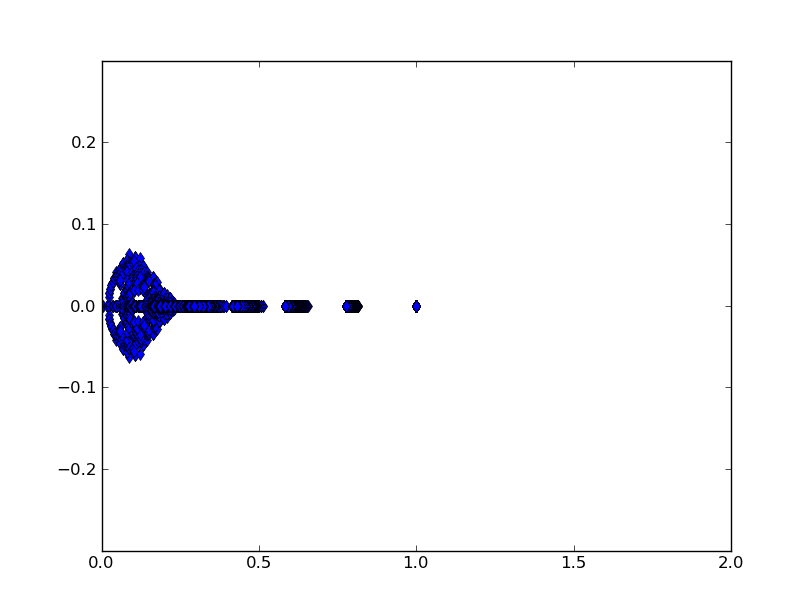
\includegraphics[width=0.5\textwidth]{./Anmg/s8_5_5}
  \caption{Eigenspectrum of the sweep preconditioned system}
  \label{eig_sweep}
\end{figure}
\begin{figure}[H]
  \centering
  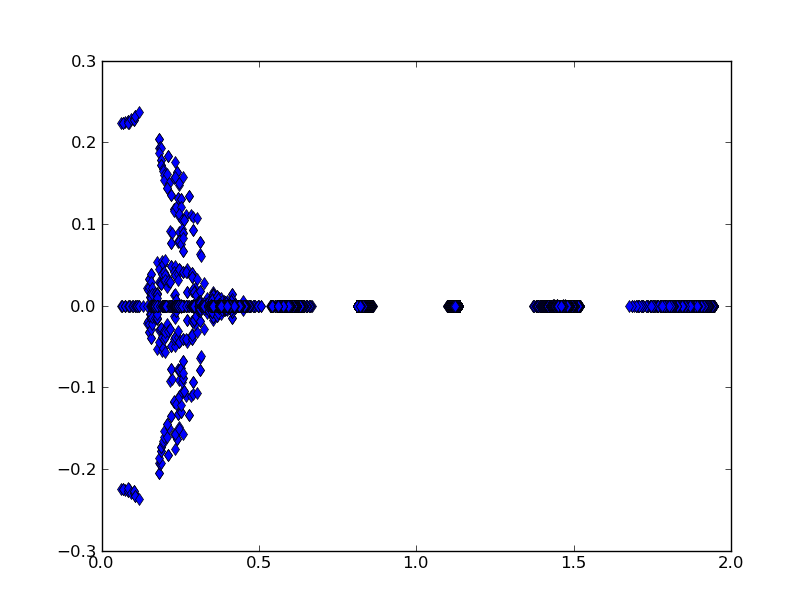
\includegraphics[width=0.5\textwidth]{./Anmg/d_s8_5_5}
  \caption{Eigenspectrum of the DSA preconditioned system}
  \label{eig_dsa}
\end{figure}
\begin{figure}[H]
  \centering
  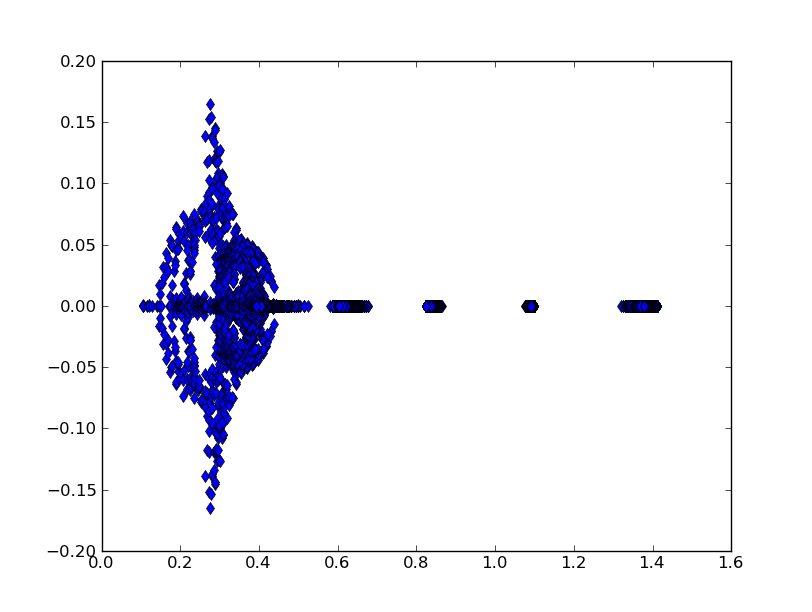
\includegraphics[width=0.5\textwidth]{./Anmg/p_s8_5_5}
  \caption{Eigenspectrum of the ANMG (DSA variant) preconditioned system}
  \label{eig_anmg}
\end{figure}
On these figures, we can note that sweep preconditioning is not effective as
many eigenvalues are located near zero. DSA moves the eigenvalues away from
zero. This explains the faster convergence of GMRES with DSA preconditioning
compared to sweep preconditioning. ANMG moves the eigenvalues even further
aways from zero than DSA and clusters them more compared to DSA. It is obvious
from these figures that ANMG preconditioning should converge much faster than
DSA preconditioning.


%\section{Algebraic Multigrid} \label{sec_amg}
\subsection{Introduction}
As mentioned earlier, the most common way to solve a SPD system is to use
conjugate gradient preconditioned with SSOR (PCG-SSOR). In this research, we
will compare the calculation time using PCG-SGS, which is PCG-SSOR with a
damping factor equals to unity, with the time needed by CG 
preconditioned with an algebraic multigrid method. This is not a new idea: the 
first multigrid methods developed were geometric multigrid used as stand-alone 
solvers. In many applications, they achieve the so-called ``textbook multigrid
efficiency'', i.e. ``the solution to the governing system of equations [is
attained] in a computational work that is a small multiple of the operation
counts associated with discretizing the system'' \cite{textbook_eff}. However, 
in many other applications, multigrid methods, and particularly algebraic 
multigrid methods, cannot achieve such efficiency \cite{k_cycle}. In
such cases, they are often used as preconditioner for Krylov subspace methods. 
AMG make  very good preconditioners because they reduce all the error modes. Of
course, some modes may not be accelerated which can significantly degrades the 
efficiency of AMG as preconditioner. In \cite{amg_pn}, the authors used an 
algebraic multigrid method to precondition the Krylov solver for the even-parity 
finite element-spherical harmonics (FE-$P_N$) method. The AMG preconditioner 
resulted in a 60\% reduction in the solution time compared to ILU(0) 
preconditioning and even more reduction compared to SSOR preconditioning. 

We will employ and compare two multigrid approaches: one from the ML package
\cite{ml_guide} from the Trilinos library and the AGMG code \cite{agmg_guide}. 
ML is a multigrid preconditioning package that uses a smoothed aggregation 
algebraic multigrid to build a preconditioner for a Krylov method. AGMG is an 
aggregation-based algebraic multigrid code (written in Fortran 90).

We describe the multigrid principles, using first a two-grid setting. Consider
the following system:
\begin{equation}
  \bs{A}_f u_f = b_f
\end{equation}
defined on the fine grid $\mathbb{T}_f$.  The two-grid algorithm is given by :
\begin{enumerate}
  \item Perform $\nu_1$ pre-smoothing iterations using a smoother (e.g., Jacobi,
    Gauss-Seidel or ILU) using an initial guess $u_0$: $u = S^{\nu_1}(u_0,b_f)$
  \item Compute the residual on the fine grid $\mathbb{T}_f$ and restrict it to
    the coarse grid $\mathbb{T}_c$: $r_c = \bs{R}(b_f-\bs{A}_f u)$
  \item Solve with a direct solver the system on the coarse grid: 
    $v=\bs{A}_c^{-1} r_c$
  \item Interpolate the coarse grid correction to the fine grid and add the
    correction to $u$: $u \leftarrow u+\bs{P}v$
  \item Perform $\nu_2$ post-smoothing iterations: $u = S^{\nu_2}(u,b_f)$
\end{enumerate}
When using AMG, the matrix $\bs{A}_c$ on the coarse grid is given by the Galerkin
approximation:
\begin{equation}
  \bs{A}_c = \bs{R}\bs{A}_f \bs{P},
\end{equation}
where $\bs{P}$ is a prolongation matrix and $\bs{R}$ is a restriction matrix.
Solving the system $\bs{A}_c v = r_c$ on the coarse grid is generally very
expansive, therefore this step is recursively replaced by $\gamma$
applications of the  two-grid
methods until the system can be efficiently inverted with a direct solver.
This yields the multigrid method. When $\gamma = 1$, respectively $\gamma =
2$, the multigrid method is said to use a $V-$cycle, respectively a $W-$cycle:
\begin{figure}[H]
  \centering
  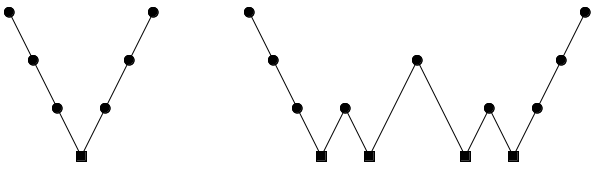
\includegraphics[width=0.5\textwidth]{./Dsa/v_w_cycles}
  \caption{$V-$ and $W-$cycles}
\end{figure}
A dot represents a smoothing operation and a square a direct inversion. The grid 
transfer operators are symbolized by lines.

For the coarsening step, both geometric and algebraic multigrid methods are 
based on the concept of smooth error. The difference between the two methods 
is that for geometric multigrid method, after the smoothing step, the error 
is \emph{geometrically} smooth relative to the coarse grid \cite{review_amg}. 
For algebraic multigrid methods, there might not be any grid and thus, only 
the properties of the matrix can be used. Therefore, the geometrical smoothness 
of the error cannot be used anymore. In fact, after the smoothing step, the 
error may be not smooth at all from the geometrical point of view. The reason 
is that the error is considered smooth when the smoother does not change the 
solution significantly anymore \cite{amg_course}:
\begin{equation}
  \|Se\|_{\mc{H}} \approx \|e\|_{\mc{H}}
\end{equation}
where $S$ is the smoother, $e$ is the error, and $\|u\|_{\mc{H}} =
\sqrt{(u,u)_{\mc{H}}}$ is the norm associated to the scalar product:
\begin{equation}
  (u,v)_{\mc{H}} = \(\bs{A}u,v\)_2.
\end{equation}
Among the algebraic multigrid methods, there are three main different 
types: the classical Ruge-Stueben AMG (also known as interpolation method), 
the plain aggregation AMG, and the smoothed aggregation AMG. ML uses 
smoothed aggregation AMG and AGMG uses plain aggregation AMG. The difference 
between theses methods is the coarsening step. The coarsening step is the 
most important step because if the coarsening is too fast, the convergence 
rates will decrease. However, if the coarsening is too slow, a lot of memory 
may be required to solve the problem. For classical Ruge-Stueben methods, 
each variable of the coarse grid is also a variable in the fine grid whereas 
for the aggregation methods, the variables of the fine grid are aggregates in
variables of the coarse grid. There is no simple identification between the 
variables of the fine grid and the coarse grid. However, all the algebraic
multigrid methods uses the  very important concept of strongly dependent
variables \cite{amg}:
{\definition{Given a threshold value of $0 \leq \theta \leq 1$, the variable
  $u_i$ strongly depends on the variable $u_j$ if:
  \begin{equation}
    -a_{ij} \geq \theta \max_{k \neq i} \(-a_{ik}\)
  \end{equation}}}
$a_{ij}$ must be of the same order of magnitude than the largest
off-diagonal in equation $i$ or $j$. A related definition is:
{\definition{If the variable $u_i$ strongly depends on the variable $u_j$,
then the variable $u_j$ strongly influences the variable $u_i$.}}\\
The idea behind the strong dependence is that if the coefficient $a_{ij}$ is
large, then a small change in the $j^{th}$ variable will have an important
effect on the $i^{th}$ variable. Thus, it is probably a good idea to use the
$j^{th}$ variable to interpolate the $i^{th}$ variable or to couple these two
variables in an aggregate. This can be easily seen using the concept of
smoothed error. For the error to be considered to be smoothed, assuming that
$\bs{A}$ is a $M$-matrix, i.e., off-diagonal entries of the matrix are less 
than or equal to zero and the real parts of the eigenvalues of the matrix 
are positive, the following relationship needs to be satisfied for most $i$ 
\cite{amg}:
\begin{equation}
  \sum_{j\neq i} \(\frac{|a_{ij}|}{a_{ii}}\) \(\frac{e_i-e_j}{e_i}\)^2 \ll 1
  \label{ineq}
\end{equation}
where $e_i$ is the error associated to the variable $i$. Since the left side 
of \cref{ineq} is positive, all the products must be small which means that 
at least one of the two terms of each product has to be small. When the
$i^{th}$ variable strongly depends on the $j^{th}$ variable 
$\frac{|a_{ij}|}{a_{ii}} \approx 1$, $e_i-e_j$ must be small
or equivalently $e_i \approx e_j$. This means that the error varies slowly
in the direction of strong connection. That is the reason why the coarsening
is done along these directions.

\subsection{Classical AMG (interpolation method)}
For classical AMG, the variables of the coarse grid are a subset of the
variables of the fine grid. The variables can be split in two disjoint
sets: $C$ that contains all the coarse variables and $F$ that contains all the
other variables. Thus, the error on the fine grid is given by \cite{review_amg}:
\begin{equation}
  e_{c,i} = (\bs{P} e_f)_i = \left\{
  \begin{aligned}
    & e_{c,i} & \textrm{ if } i\in C\\
    & \sum_{k\in B_i} w_{ik} e_{c,k} & \textrm{ if } i\in F
  \end{aligned}
  \right.
\end{equation}
where $B_i$ is a subset of $C$ whose variables are called interpolatory
variables. $B_i$ should be a small subset of $C$ to keep $\bs{A}_c$ sparse.
Now, we assume that $\bs{A}$ is a $M$-matrix and we review two typical 
interpolation methods:
\begin{description}
  \item[Direct interpolation:] First, we define the neighborhood of the
    $i^{th}$ as the set $N_i = \{ j \in C \cup F: j\neq i, a_{ij} \neq 0\}$.
    After the smoothing step, we can write locally:
    \begin{equation}
      e_i \approx -\frac{\(\sum_{j\in N_i} a_{ij} e_j\)}{a_{ii}}.
      \label{e_locally}
    \end{equation}
    If $B_i$ contains the variables which are strongly dependent on the
    $i^{th}$ variables, we have:
    \begin{equation}
      \frac{1}{\sum_{k\in B_i} a_{ik}} \sum_{k \in B_i} a_{ik} e_k \approx 
      \frac{1}{\sum_{j\in N_i} a_{ij}} \sum_{j \in N_i} a_{ij} e_j.
    \end{equation}
    Using this relation and \cref{e_locally}, we get the following formula for
    the weights of the interpolation:
    \begin{equation}
      w_{ik} = -\alpha_i \frac{a_{ik}}{a_{ii}}
    \end{equation}
    where $\alpha_i = \frac{\sum_{j\in N_i} a_{ij}}{\sum_{l \in B_i} a_{il}}$.
    Therefore, it is important that when the coarse variables are chosen,  
    that every variable in $F$ has enough strongly coupled
    variables in $C$ that are part of of $B_i$. If some of the off-diagonal
    entries are positive, the same development can be done as long as these
    positive terms are small, i.e., variables are not strongly coupled because
    of these terms. If the positive entries are large, the algebraically
    smooth error can oscillate. This can happen, for elliptic PDE, when 
    high-order finite elements are used or with bilinear elements on 
    quadrilateral meshes with large aspect ratios. This will negatively affect
    the performance of AMG.
  \item[More complex interpolations:] More complex interpolation schemes can
    be created but they reduce the sparsity of $\bs{P}$ and $\bs{R}$, increasing the
    size of $\bs{A}_c$. Moreover, the weakly-dependent variables will be 
    associated to smaller weights which makes them having a small effect. It
    can therefore be interesting to ignore the smallest values in the
    interpolation matrix and to rescale the others weights so that the sum of
    the weights does not change. This can slow down the convergence of the
    method but it will not make it diverge \cite{review_amg}.
\end{description}
A good rule, when coarsening the grid, is to try to have the set of coarse 
variables to form a maximally independent set, i.e. a maximal set where the 
coarse variables are not strongly coupled to each others, and the variables 
in $F$ are surrounded by the variables in $C$. We call $B_i^S$ the set of all 
strongly connected neighbors of $u_i$:
\begin{equation}
  B_i^s = \{ v_j \in B_i | -a_{ij} \geq \theta \max_{k\neq i}(-a_{i,k})\}.
\end{equation}
The interpolatory nodes $C_i$ are:
\begin{equation}
  C_i = B_i^s \cap C.
\end{equation}
Adding variables in $C_i$ increases the quality of the interpolation but
it diminishes the sparsity of the interpolation matrix and increases the
size of $\bs{A}_c$ which increases the computational cost of the method.
Thus, we want that for every variable $u_i$ in $F$, every $u_j \in B_i^s$
should be in $C_i$ or strongly connected to at least one variable in
$C_i$. This rule will make sure that the interpolation is of a good enough
quality. We also want $C$ to be a maximal subset of the variables such that 
the variables in $C$ are not strongly connected to each others. This ensures 
that the coarsening is fast enough.

\subsection{Smoothed aggregation: the ML package}
In a similar way than for the classical AMG, the smoothed aggregation
method uses the concept of strong connections. The theory for plain
aggregation method showed that the convergence bound depends of the number
of levels \cite{amg_unstruc}. This is a major flaw of the plain aggregation
method which was also observed in practice. To counter this, the smoothed
aggregation was created. This method converges fast for a lot of different 
problems including the ones with anisotropic and discontinuous coefficients.
  
When using a smoothed aggregation scheme, the smoothed interpolation operators,
$\bs{P}_k$, are the transpose of the coarsening operators,
$\bs{R}_k=\bs{P}_k^T$. Therefore, when the $\bs{P}_k$ are built, the
coarsening is known. First, the graph of the matrix is constructed: if the element
$(i,j)$ or $(j,i)$ of the matrix is non-zero, an edge is built between the
vertex $i$ and the vertex $j$ \cite{ml_guide}. Second, the vertices are
aggregated. When using ML on a single processor, two aggregation schemes can
be used: the uncoupled scheme or the maximally independent sets (MIS) scheme. 
The uncoupled scheme attempts at building aggregates of size $3^d$ where $d$ is the
dimension of the problem. The algorithm works as follows \cite{mis}:
\begin{description}
  \item[Step 1:] As long as there are points not adjacent to an aggregate:
    \begin{enumerate}
      \item Choose a point which is not adjacent to an aggregate. This point
        is a new root point.
      \item Define a new aggregate as the root point and its neighbors.
    \end{enumerate}
  \item[Step 2:] Add all the points left to the existing aggregates or form a
    new aggregates with them.
\end{description}
The MIS scheme used in ML applied the MIS algorithm of \cite{graph_coloring} to
the graph produced by the matrix $\bs{A}^2$. These two coarsening 
schemes use a fixed ratio of coarsening between levels. Once the aggregation is 
done, a tentative prolongator matrix, $\bs{\tilde{P}}_k$ is constructed 
\cite{mis}. A example of $\bs{\tilde{P}}_k$ is given by:
\begin{equation}
  \bs{\tilde{P}}_k(i,j) = \left\{
  \begin{aligned}
    &1 &\textrm{if }i^{th}\textrm{ point is contained in }j^{th}\textrm{
    aggregate}\\
    & 0 &\textrm{otherwise}
  \end{aligned}
  \right.
\end{equation}
This tentative prolongator could be used as prolongator but smoothing it
allows to have a more robust scheme. Let $\bs{S}_k$ be a smoother, for example
damped Jacobi, then the prolongator matrix is given by:
\begin{equation}
  \bs{P}_k = \bs{S}_k \bs{\tilde{P}}_k.
\end{equation}

Like for classical AMG, it can be interesting to ignore small values in
the graph since the smoother will be ineffective for the weakly coupled
variables. In ML, there is a drop tolerance, $tol$, that is used to ignore
entries in the graph if $|a_{ij}| \leq tol\ \sqrt{|a_{ij} a_{jj}|}$. The
tolerance, whose default value is zero, can be changed.  In ML, when the 
matrix is SPD, CG is used to determine the Jacobi damping parameter, which 
is an approximation of the spectral radius.

By default, the coarsening is stopped when the number of variables is less 
or equal than 128.

\subsection{Plain aggregation: the AGMG code}
Unlike ML, in AGMG the prolongator is not smoothed which results in a
cheaper setup and a decrease of required memory \cite{agmg2}. However, 
the scheme could be less robust. To counteract this weakness, 
the aggregation scheme is more complicated. Coarsening algorithms that control
the size of the aggregates tends to produce a few badly shaped aggregates.
Since the convergence of AMG is bounded by the worst aggregate, even a small 
number of badly shaped aggregates can have a huge impact on the convergence. 
In AGMG, the aggregation algorithm has as input the upper bound of the 
two-grid condition number $\bar{\kappa}_{TG}$. When the aggregates are constructed,
their quality is checked. Obviously, this increases the cost of the coarsening
and it is important that the coarsening is fast enough. Since the algorithm 
does not control the size of the aggregates, it is difficult to control the 
speed of the coarsening. However, controlling the condition number is much 
more interesting than controlling the coarsening speed. If the algorithm 
controls the condition number, it will not create bad aggregates but instead, it 
may create a few aggregates with a size below the target size but this 
does not affect the efficiency of the method in a noticeable way \cite{agmg2}. 

In AGMG, the aggregation is done by a few passes of a pairwise aggregation 
algorithm. This allows the computation of the aggregate quality to remain very 
simple and to keep the cost per iteration low. The advantage of controlling the 
condition number becomes even more important when a $K-$cycle or Krylov-cycle is 
used instead of the more common $V-$ or $W-$cycles. The difference between the 
$K-$cycle and the $V-$ or $W-$cycle is that the $K-$cycle uses recursively a 
few iterations of a Krylov solver preconditioned by a coarser grid to solve 
the coarse grid problem in the two-grid algorithm \cite{k_cycle}. This scheme 
is nonlinear and requires, when the system is SPD, to use flexible CG 
\cite{fcg_2,fcg_3,fcg_4,fcg} as Krylov solver. The advantage of the $K-$cycle is 
an increased robustness compared to $V-$ and $W-$cycle. Even when the condition 
number of the two-grid method is large, the convergence properties of the 
$K-$cycle can be independent of the number of levels \cite{k_cycle}. The 
computational cost of $K-$cycle is about the same than the cost of the 
$W-$cycle. If the number of unknowns does not decrease sufficiently from one 
level to the next, the $K-$cycle at one level is replaced by a $V-$cycle at 
this same level. The idea of $K-$cycle is not new since it was already used 
in Algebraic MultiLevel Iteration (AMLI) methods \cite{amli}. AMLI are 
hierarchical basis methods stabilized by the recursive calls of preconditioner 
created thanks to a coarse level. 

Next, we explain the coarsening step in AGMG for $M-$matrix (SPD). 
We want to create nonempty disjoint sets $G_k$, $k=1,\hdots,n_c$ called 
aggregates with each one of them associated to a variable in a coarser grid. 
Some of the unknowns are not associated to any variables in the coarse grid 
and they are in the set $G_0$. The prolongation matrix is given by:
\begin{equation}
  \bs{P}_{ij} = \left\{
    \begin{aligned}
      1& \textrm{ if }i\in G_j\\
      0& \textrm{ otherwise}
    \end{aligned}
    \right.
\end{equation}
Thus, $\bs{P}$ has at most one non-zeros entry by row. A row is only
composed of zeros if the variable associated to this row is in $G_0$. A
simple method to form the high quality aggregates of a given size would be
to test all the possibility. For an obvious reason, this cannot be done in
practise. Instead, in AGMG several passes of pairwise aggregation are done. 
The reason is that when two variables are aggregated, the quality factor of 
the aggregate $\kappa(G)$ is given by: 
\begin{equation}
  \kappa(\{i,j\}) = \frac{-a_{ij} +\(\frac{1}{a_{ii}+s_i+2a_{ij}}+
  \frac{1}{a_{jj}+s_j+2 a_{ij}}\)^{-1}}{-a_{ij}+\(\frac{1}{a_{ii}-s_i}+
  \frac{1}{a_{jj}-s_j}\)^{-1}}
\end{equation}
where $s_i = - \sum_{j\neq i} a_{ij}$. $\kappa$ is only given by the
off-diagonal entry connecting these two unknowns, their respective diagonal
entries, and the sum of all off-diagonal elements in the corresponding rows.
As $|G|$ increases, it becomes more and more costly to compute
$\kappa(|G|)$. However, checking that $\kappa(|G|)$ is below a given
threshold $\bar{\kappa}_{TG}$ is relatively cheap. It is sufficient to
check that:
\begin{equation}
  \bar{\kappa}_{TG} \bs{A}_G - \bs{M}_G\(\bs{I}-\bs{1}_G \(\bs{1}_G^T
  \bs{M}_G\bs{1}_G\)^{-1}\bs{1}_G^T\bs{M}_G\)
\end{equation}
is nonnegative definite. This can be done in $\mc{O}(|G|^3)$ operation
by verifying that the Cholesky factorization exists, i.e., there is no negative
pivot. Therefore, $\kappa(|G|)$ does not need to be computed explicitly to
make sure that $\kappa(|G|) \leq \bar{\kappa}_{TG}$. The first pairwise
coarsening step is given by:
\begin{enumerate}
  \item Create the set $G_0$, i.e., create the set of variables which will
    not be aggregated.
  \item Choose an unknown and find among its unassigned neighbors the one
    that gives the smallest $\kappa(\{i,j\})$.
  \item Check that $\kappa(\{i,j\}) \leq \bar{\kappa}_{TG}$. If the
    condition is not verified, the variable is left unassociated in the coarse
    grid.
\end{enumerate}
To increase the size of the aggregates, the temporary coarse grid matrix
$\bs{\tilde{A}}_c$ is computed and the same process that the one we just
described is applied. The set $G_0$ cannot be changed and the quality factor
$\tilde{\kappa}(\{i,j\})$ needs to be adapted to reflect the quality of the
corresponding aggregate $\kappa(G_i\cup G_j)$ in the original matrix.
Therefore, the definition of $s_j$ is slightly modified:
\begin{equation}
  \tilde{s}_i = - \sum_{k \in G_i} \sum_{j \in G_i} a_{kj}.
\end{equation}
This change is there to ensure that $\tilde{\kappa}(\{i,j\})$ is a lower
bound of $\kappa(G_i \cup G_j)$. Thus, if $\tilde{\kappa}(\{i,j\}) \geq
\bar{\kappa}_{TG}$, the pair has to be rejected because it is impossible for
$\kappa(G_i \cup G_j)$ to satisfy the condition. An unique characteristic 
of this coarsening method is that you can, in theory, have an 
arbitrary number of pairwise coarsening passes without degrading the upper
bound of the condition number. In practise, however, the coarsening is
stopped if either a given number of passes has been done or the coarsening
factor has reached a target value. To conclude the explanation of the
coarsening step, we explain how unknowns are picked and how to pick between 
a pair $\{i,j\}$ and another $\{i,k\}$ if they have the same quality factor. 
If there is no priority rules, the coarsening would depend of the ordering 
of the variables or the way off-diagonal entries are stored. In AGMG, the 
rule chosen tries to increase the regularity of the aggregates because in 
practise, this increases the coarsening speed of the coarser levels. Even 
if the coarsening step tries to create regular aggregates on regular grids, 
the results are still quite good for unstructured grids \cite{agmg2}. The 
priority rule consists of using a Cuthill-McKee permutation 
\cite{cmk} to renumber the variables and to use the number associated to the 
variable as a priority number (the lower number has the priority). The 
Cuthill-McKee permutation works as follows: the number 1 is given to a node 
with minimal degree; the next numbers are given to its neighbors ordered by
increasing degree; then their neighbors are given a number by
increasing degree; the process is over when all nodes are numbered. There is
still some uncertainties in the numbering if there are several variables
with minimal degree or when several neighbors of a variables have the same
degree. However, these choices do not affect the
performance \cite{agmg2}. 

AGMG stops the coarsening when the number of variables is less or equal to
400.


% bibliography
\bibliographystyle{unsrt}
\bibliography{biblio}
% include all the references
%\nocite{*}

\end{document}

